\newpage
\section{Experiments}

% 1) Very quick summary of the modelling tasks
% goal: use 2 types of tasks - graph classif and node regression
%       try some of the models
%       find a novel solution to a problem
% organization: the tasks selected are G-N approximation and  
The goal of this master's thesis is to apply Graph Neural Network models to different problems to create a novel solution. The idea is to get to know how Graph Neural Networks are used in each situation. Two problems are explored: Girvan-Newman algorithm approximation and compiled code function classification. They correspond to the two main tasks that Graph Neural Network perform with success, semi-supervised learning of nodes on a graph and supervised graph classification. 

This section will present the configuration of the experiments performed in the thesis. First, the Girvan-Newman approximation experiment is explained. Then the compiled code function classification experiment is described last. In each case, context, goals and motivation are described first. Then a preliminary test is performed on well-known benchmark datasets to verify the in use works correctly in the computer without any problem. Then the process of data preparation is explained and finally how the part of training a model is executed is summarized.

% 2) Girvan-Newman approximation
\subsection{Girvan-Newman algorithm approximation}

% 2.1) Girvan-Newman: description (review state of the art quickly),
\textbf{Context} 
The Girvan-Newman algorithm is a clustering based approach to perform community detection. It proposed a divisive algorithm based on edge-betweenness for a graph with undirected and unweighted edges. The algorithm focused on edges that are most "between" the communities and communities are constructed progressively by removing these edges from the original graph. It iteratively isolates groups of nodes of a graph by removing the edges that poses the greater edge betweenness value. The worst-case for time complexity of the edge-betweenness algorithm is $O(m^2n)$ and is $O(n^3)$ for sparse graphs, with $m$ being the number of edges and $n$ the number of vertices. 

\textbf{Goal}
%          goal (approximate it), 
The goal of this experiment is to find a novel way to approximate the Girvan-Newman algorithm that is faster than the original.


\textbf{Motivation}
% motivation find a good balance point between speed and accuracy, 
The motivation is simply to find a faster but approximated implementation of an algorithm that is popular for community detection tasks. At the same, community detection is a popular task with applications in many areas related to social network analysis.


\textbf{Experiment overview}
%actual ideas for approximation
To be more precise, the function to approximate will be the computation of the edge betweenness for each edge of the graph in each iteration of the algorithm. Thus, the experiments will focus solely on finding a Graph Neural Network that approximates the computation of the edge betweenness with a reasonable performance.

% edge betweenness definition
For any node in a graph, node betweenness is defined as the number of shortest paths between pairs of nodes that run through it. The Girvan–Newman algorithm extends this definition to the case of edges, defining the "edge betweenness" of an edge as the number of shortest paths between pairs of nodes that run along it. If there is more than one shortest path between a pair of nodes, each path is assigned equal weight such that the total weight of all of the paths is equal to unity.

There are two main ways to approximate the edge betweenness with Graph Neural Network models. 

The first one, using supervised learning for doing node attribute value regression. A model will be trained to approximate the edge betweenness of all edges of a graph. The final approximated Girvan-Newman algorithm would consist of the original process but replacing the computation of the edge betweenness by the trained model.


%               1) approxima edge_betweenness of all the nodes in each iteration of GN
% 				2) in each iteration, compute edge -betweenns of some nodes, then use GCN in a transductive setting to expand to the rest of nodes(hopefully faster)
In the second approach, by using semi-supervised learning, one can compute the edge betweenness of several nodes and then train the model to predict the value for the rest of edges of the graph. In that case, the Girvan-Newman algorithm would, in each iteration, first compute the edge betweenness of some edges in the normal way, then use the model to approximate the edge betweenness of the rest of the edges of the graph. By the nature of the Graph Neural Networks that have attained state-of-the-art performance on semi-supervised learning, the second approach seems the most realistic one.


\textbf{Preliminary test}

As a way to verify that available code from published research works correctly on computer on which the experiments will be performed, a published experiment is reproduced. A task of semi-supervised classification is reproduced locally, training a set of GCN, ChebNet, GAT , SG and APPNP models. The Cora dataset is used for this task.  The Cora dataset consists of 2708 scientific publications classified into one of seven classes. The goal is to verify that the computer that will support the experiments can train those models without memory problems or other types of problems. Also it is a way to check that some configurations of hyper-parameters yield good results for later comparison with the real experiments. 


% 2.2) data gathering process
\textbf{data preparation:}


\textbf{Datasets used}
%  collection process(Pytorch Geometric dataloader)
%  types of graphs used
For the Girvan-Newman aproximation experiment, well known datasets available from Pytorch Geometric library are used:
\begin{itemize}
	\item Proteins,
	\item PPI,
	\item QM7,
	\item WS random generated graph,
	\item and Karate-Club.
\end{itemize}

\textbf{Data preparation}
%  data inspection(None)
%  precomputation of the edge-betweennes for target preparation
The experiment is focused on training a Graph Neural Network that will approximate the edge betweenness. 

For that purpose, there's different ways to handle graphs on a dataset. The reason is the following, for training  a model for predicting the edge betweenness of an edge, some parts of a graph are used as training, validation and others as testing. This implies that a small graph will produce dataset splits that contain few edges and so the model trained on those small subgraphs usually won't be able to learn a good approximation. For that reason, the datasets that contain  several small graphs are treated as a big graph with disconnected components. When the dataset contains only one graph, it will usually be big and so the sub graphs splits for training, validation and testing will be enough in size for the model to train properly.

The setup of the target value, the ground truth value of the edge betweenness of each edge of the graph, will be specific to the how the graphs of a dataset are handled. When there's only a graph on the dataset, it is straight forward to compute the edge betweenness of each edge from the NetworkX graph library and used it as the ground truth(the target value) for the model training. When the dataset contains many separated graphs, there are two ways to approach the experiment. The first way is to process all graphs together as if it was a big graph with disconnected components and compute the edge betweenness in this setup. The second way is to process all graphs together as a big graph with connected components but to compute the edge betweenness for each graph alone. 


Since Graph Neural Network models available are only prepared to learn representations of nodes, that is, learn a node state formed by node attribute values, we transform the problem of computing the edge betweenness of edges into the problem of computing the node betweenness of an equivalent graph where the nodes are transformed to edges and the edges are transformed to nodes. This transformation is performed on the dataset, where for each graph, the list of nodes and the list of edges is transformed accordingly. 

\textbf{Experiments}
% 2.3) Experiments list (main task and side analysis)
%  GCN training
%  graphSage training

The experiments consist in training several types of models on the task of predicting the node betweenness of a derived graph from the original dataset, using the previous listed  datasets. The types of models are variations of GCN and GraphSAGE implemented in PyTorch Geometric python library:
\begin{itemize}
	\item GCN, GraphSage, ChebNet or Gated Graph Neural Networks
	\item some fully connected layers at the end
\end{itemize}
Based on this architecture, different adjustments on the number of layers, the number of units of layers, and other hyper parameters will be modified during hyper-parameter search.

If this experiment does not attain an acceptable performance, it will be modified into aproximate other graph measures like node betweenness centrality or PageRank.

Another variation of this experiment, could be to transform the regression nature to a classification setup, where the graph measure of interest is divided in ranges and the model is trained to classify each node or edge feature into one of the available ranges

\textbf{Evaluation procedure}
%  inspecting the distribution of results
To evaluate the results, the performance metric used is the Normalized Root Mean Squared Error (NRMSE). 

As a complement to understand how performant a model is, the distribution of predicted values versus their true target values is compared in a scatter plot. The cloud of points is plotted in the 2D, to be able to see if if deviates from the 45º line (y=x line). \\
\\




\subsection{Compiled code function classification}
% 3) Function renaming

\textbf{Context}
% 3.1) Function renaming: 
%  description: quick recap of sota about code2vec and varnaming tasks
There have been some research publications related to the topic of program analysis. As mentioned in the section 2, there have been approaches to classify code snippets \cite{code2vec} and variables \cite{139} and their usage so that a name can be assigned to them. 

\textbf{Goal}
%  goal: apply those same tasks to compile code (assembler)
Inspired by those examples, the second experiment of this thesis tries to create a predictive model that will classify a snippet of code in assembler language, the programming language that has a direct transcription to machine code in compiled binaries. The experiment will focus on entire functions or subroutines in assembler language. The experiment will not try to replicate any of the conditions of the research that inspired it, since this experiment will be performed on a different programming language than \cite{139} and \cite{code2vec} and a different kind of model than \cite{code2vec}.

\textbf{Motivation}
%  motivation: reverse engineering for malware(malicious code) analysis (process steps, where the algorithm could help)
%              what is the decision on the precise goal: main functionalities(crypto, network, disk, ..)
This experiment could build a classification model that is useful for professionals that work on anti-virus companies. In any anti-virus company, there are security engineers that analyze malicious code, also called computer virus or malware. Part of the process of analyzing a malicious code consists in reverse engineering the code contained inside a binary file. Besides fighting against code obfuscation techniques, the reverse engineer is faced with several thousands of assembler subroutines or functions that he needs to inspect to find where the important code functionalities reside. One way to proceed is from the hints of the interaction of the malicious code with its environment. When a malicious code reads files or connects to Internet urls, called artifacts, the reverse engineer can begin to trace back the functions that use those artifacts. In the process of tracing the code related to those artifacts, or in looking for main actions like connection to the Internet, the reverse engineer will write comments, annotate code snippets or rename functions.
It is estimated that having an indication of the main functionality that a code snippet performs can help reverse engineers to find more quickly the evidences the need when analyzing malicious code. This indication can be implemented as renaming the functions of a binary. The renaming of a function can be based on the classification that a machine learning model will predict on it.



\textbf{Experiment overview}
%  overview of the process: building the dataset, transform it, label it, preprocessing, then training the models
The experiment consists in several complex steps.
First, building a dataset that is suitable for training a model on classifying code on a set of predefined classes. Some binaries that contains functions related to the chosen predefined classes are collected from open source software.  
Next, those binaries and their functions are analyzed by a program that translates machine code to assembler language. This kind of tool is called a disassembler.
Then, different representations of those functions in assembler have to be generated: a graph for each function and some features related to the assembler code itself and to the structure of the graph.
After that, the collected dataset must be correctly labeled. Since the intent is to train a model in a supervised setting, each function (corresponding to a sample of the dataset) must be labeled with one of the predefined classes.
Finally, with the dataset correctly labeled and with all its features in place, the models can be trained to classify assembler code functions. A set of baseline classification models, then some basic NLP models and finally a set of GNN models will be trained. 


\textbf{Data preparation}
% 3.2) data gathering process

Let's first review the complex data preparation process. There's no open source dataset with the properties needed for the experiment so it will be created from scratch.



\textbf{Data sources}
% sources of compiled code: malware samples(why not?  unlabeled and on top of it obfuscated)
%                           well-known softare: webservers, cryptographic libraries, disk utilis,  copyright protection software
Since the main audience could be malicious software analysts, one possibility of getting data from would be to collect analyzed malicious code. It turns out that there's not many sources of analyzed malicious code, and also, malicious code is plenty of obfuscation techniques, which would be an entire different experiment to deal with. 

Instead, the preferred strategy is to use well-known software that contains the functionality according to the predefined classes. A decision was need to be made on the set of labels that the dataset will contain. A set of main functionalities related to general purpose applications would be:
\begin{itemize}
	\item network
	\item cryptography
	\item disk access
	\item memory manipulation
\end{itemize}
According to that list, several open source tools and libraries are collected, in order to have at least several binaries in each of the previous categories. To that end, open source binaries from web servers, email clients, ftp servers and clients, cryptographic libraries, disk utilities and C library are collected.





\textbf{Data transformation}
% data transformation: plugin to extract assembly code as a graph. 
For generating the dataset, a plugin in Python programming language has been developed to be used inside a disassembler program, namely the free version of IDA, a popular professional disassembler program.


% abstract idea - each instruction/register/memaddr... is a node
% in which instruction it is used is a vertex
% 									  order of executions of instructions form vertex between then + branchs/calls/loops...
%									NetworkX format from txt files 
This plugin visits all the functions detected in a binary and extracts the information of instructions, operands and cross-references to generate a graph of the relationship between them. Every instruction, operand, memory address or constant is a node of the graph. Every relationship between them is a vertex of that graph. There's worth mentioning that instructions are executed one after another and so usually an instruction will be linked to its previous and next instruction in the execution flow. However, sometimes loops, conditional branches and function calls modify this sequential execution flow.

The graph is saved in a format suitable for the Python library NetworkX to read it and import it. The format consists of 2 text files, one with the list of nodes and their attributes, the other with the list of edges and their attributes.


% data transformation for baseline models: summary statistics of graphs, and other topological features
% data transformation for nlp models: Bag of words with TF-IDF
Besides from the graph representation of each function of a binary file, the attributes that will be used by baseline models are also generated. There are topological features from the graphs and features extracted directly from the code itself, like the Bag of Words embedding (fined tuned by TF-IDF).




\begin{figure}[H]
    \centering
        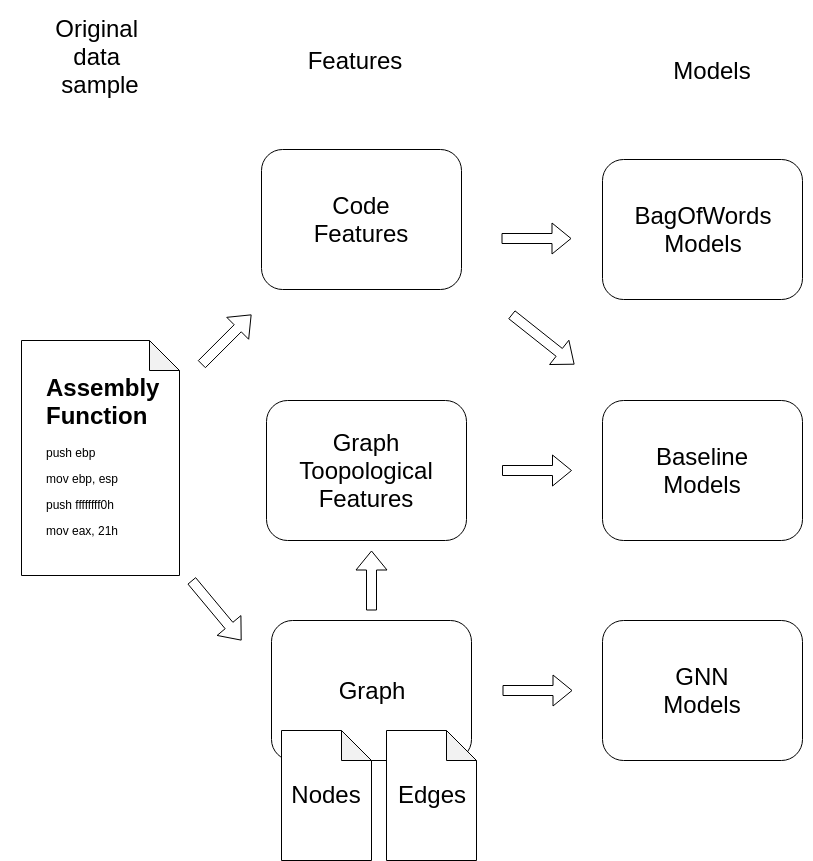
\includegraphics[width=0.55\linewidth]{img/Features_and_models_diagram.png}
    \caption{Features exracted from the dataset samples and their relationship with the models trained}\label{fig:Features_diagram}
\end{figure}

All of these features and graph representation will be transformed into a Dataset module from Pytorch Geometric library. This will allow the training of Graph Neural Network models to use the complete ecosystem of PyTorch Geometric for loading graphs, training models and test their performance.




\textbf{Supervised labels generation}
% 3.3) labelling discussion
		% approach1: all assembly code from a binary under the same label
		% approach2: compile with symbols and then infer label from function name
		%            rules: topics and tasks, 
		%            final sets of labels v1,v2,v3


In the first approach, it was decided that all functions of a binary will be labelled with the main purpose of the binary. For example, all functions of a web server would be labelled network. This approach is too coarse grained and therefore may lead to useless classification models.
 
A second approach would consist in obtaining the open source software sources and then compiling it with debugging information. This type of compilation maintains the original function names that developers assigned to functions. Then after obtaining the assembler code of each functions and its original name, some simple rule where created to derive a label from the function name. Basically the appearance of keyword would drive this process. Additionally,human supervision has been applied to improve the labeling assignments. 

Four different versions of the dataset have been generated:
\begin{itemize}
	\item v0: each binary and all its functions have the same label. A coarse grained and noisy approach
	\item v1: 10 different labels have been chosen, and function labels has been assigned by keyword appearance in the debugging information (original function name)
	\item v2: a list of topic and tasks has been compiled and combined to generate 120 different labels. Keyword appearance rules and human supervision have been used to assign labels
	\item v3: a reduced list of topic and tasks has been compiled and combined to generate 24 different labels. Keyword appearance rules and human supervision have been used to assign labels
\end{itemize}
The idea was to find the correct granularity of the dataset. Trained models tend to perform better in the smaller sets of labels (v0 and v1), but there is the risk that the model does not capture any of the information of interest. 



\textbf{Model trainings}
% 3.4) Experiments list (each attempt with different datasets, baselines, nlp and ggnn)

The experiments performed in this second tasks are first, a reproduction of some of the results in graph classification tasks by Graph Neural Networks to make sure that we are able to attain a similar performance with the tools at hand (Pytorch implementation of Graph Neural Network components). Second, the baseline and graph neural network models will be trained on the datasets v0 to v3. 

\textbf{Graph classification benchmark}
% graph classification experiment reproduciblity
The graph classification tasks on the datasets Enzymes, Proteins, IMDB binary and QM9 are reproduced with different model architectures than the ones on the benchmarks of Pytorch Geometric library. The results are based on the f1-macro average score.




\textbf{Compiled code classification models}
% function renaming experiments

% baseline models training (noisy,v1,v2,v3)
% nlp models training      (noisy,v1,v2,v3)
% gnn models training      (noisy,v1,v2,v3)

A set trainings will be performed on baseline models, Bag-of-word models and GNNs.

The set of baseline models used are:
\begin{itemize}
	\item Logistic Regression
	\item Decition trees
	\item Random Forest
	\item XGBoost
	\item MLP (Multi-layer perceptron)
\end{itemize}

The set of Bag-of-words models consists of the baseline models of the previous list, but using the bag-of-word tfidf embedding as an input. There will also be mixed features from topological features or code features, concatenated with the embeddinf from tfidf.

The set of Graph Neural Networks used consists of combinations of:
\begin{itemize}
	\item pooling layers to reduce dimensionality
	\item GCN, GraphSage or Gated Graph Neural Networks
	\item global pooling to extrat a graph level set of attributes
	\item some fully connected layers at the end
\end{itemize}

Based on this architecture, different adjustments on the number of layers, the number of units of layers, and other hyper parameters will be modified during hyper-parameter search.



\textbf{Evaluation}
To evaluate model performance, the f1-score with a macro average will be used. F1-score allows to measure precision and recall at the same time (it's the harmonic mean). Macro averages in an imbalanced context allow for the performance to be measure as if all classes should be equally performant. Macro averages protect the training of the model from the possibility that it learns to classify only the majority class.